
%---------------------------------------------------------------------
%
%                          capítulo 4
%
%---------------------------------------------------------------------

\chapter{Tecnologías empleadas}
\label{cap4:sec:capitulo4}

En este capítulo se presentan las tecnologías y dispositivos empleadas para el desarrollo del proyecto. Detallando de forma técnica el \textit{software} y \textit{hardware} utilizado.

\section{Software empleado}

Para el desarrollo de este proyecto, el principal software utilizado ha sido \texttt{Unity 2019.4.9f1}\cite{Unity_Manual}. Este \textit{Game Engine} hace referencia a una plataforma de desarrollo de software capaz de realizar rutinas de programación que permiten el diseño, la creación y el funcionamiento de un entorno interactivo;

Con el fin de elaborar, compilar y depurar el proyecto de \texttt{Unity} se ha utilizado \texttt{Visual Studio 2019}\cite{ VisualStudio} con el lenguaje de programación C\#, ya que mantienen una sola base de código para todas las plataformas. Respecto a la creación de los personajes, se observó que \texttt{Fuse Character Creator de Mixamo}\cite{FuseCharCreaMixamo} ofrecía una  creación de modelos humanos realistas con una alta calidad de las texturas. En cuanto a la configuración previa de las animaciones, se hizo uso de \texttt{Mixamo 3D Animation Online Services}\cite{Mixamo3DAnimation}, ya que es una compañía tecnológica encargada del desarrollo y venta de servicios para la animación de personajes 3D. Como plataforma para el desarrollo colaborativo del proyecto se usó GitHub, utilizando el sistema de control de versiones Git.

\subsection{Unity}
\label{cap4:sec:unity}

El objetivo de este proyecto trata de como poder realizar una captura de movimiento de calidad sobre el arte marcial afrobrasileño (capoeira) y como representarla gráficamente con las tecnologías más demandadas del mercado.

Un \textit{Game Engine} se especifica como la rutina de programación que permiten el diseño, la creación y la representación de un videojuego. La funcionalidad de un motor de videojuegos consiste en, proveer al desarrollador un motor de renderizado para la creación de gráficos 2D y 3D, un motor físico, sonidos, scripting, animaciones, un escenario gráfico, etc.

Para llevar todo esto a cabo es necesario elegir qué tipo de plataforma de \textit{Game Engine} utilizar en este proyecto. Existe dos grandes plataformas comerciales, por lo que la decisión de elegir entre \texttt{Unity}\footnote{\url{https://unity.com/}} o \texttt{Unreal Engine}\footnote{\url{https://www.unrealengine.com/}} fue basada en la comunidad que hay detrás de cada uno de ellos, y sobre todo, en lo que se quiere abarcar con este proyecto.

Además de este detalle, es importante conocer el lenguaje de programación con el que trabaja cada uno de ellos. \texttt{Unity} está basado en \texttt{C\#}, mientras que \texttt{Unreal Engine} trabaja con C++.

La versatilidad de \texttt{Unity}, ideal para proyectos pequeños, estudiantiles o enfocados al desarrollo de aplicaciones y juegos para móviles, ha conseguido que un 58\% de la población de desarrolladores indies lo elijan como motor de videojuegos. Las facilidades que aporta a la hora de trabajar de una forma visual y escalable lo convierten en un paso muy a tener en cuenta a la hora de realizar desarrollos enfocados a la creación de entornos 3D.

En este caso \texttt{Unity}, se adecua correctamente, ya que se pretende realizar un entorno 3D donde los usuarios perciban y aprendan movimientos del arte marcial afrobrasileño.

En un primer momento, \texttt{Unity} salió al mercado ofreciendo un \textit{software} de calidad y barato, añadiendo el objetivo de que pequeñas y grandes empresas pudieran utilizarlo por igual, dando además, la posibilidad de que su contenido sea compatible con prácticamente cualquier medio o dispositivo\cite{Unity-relations}. Gracias a ello, \texttt{Unity} creció exponencialmente en el mercado, generando así, una gran comunidad que puede servir de pilar de ayuda para los nuevos desarrolladores.

Como en otras plataformas de desarrollo de software, existen distintas licencias de prueba gratuitas y para estudiantes a las que puedes acceder sin complicaciones. Sólo aquél que realmente decida llevar su creación al mercado y supere cierta cantidad de ingresos se verá obligado a pagar la cuota mensual. En la versión personal (licencia gratuita), es necesario promocionar el logotipo de \texttt{Unity} cuando se inicia la aplicación una vez compilada.

Otro aspecto importante de \texttt{Unity} es el \texttt{Asset Store}. Se trata de una biblioteca, que contiene una multitud de paquetes o \textit{Assets} comerciales y gratuitos, creados de forma continua por la comunidad, por \texttt{Unity Technologies} o empresas de terceros. Estos paquetes pueden contener modelados 3D, texturas, animaciones y demás contenido que sirva de ayuda para desarrollar un proyecto donde ya sea por tiempo o habilidades técnicas, no sea posible desarrollar cada una de la herramientas que ofrece dicha tienda.

La plataforma para el desarrollo de este proyecto, \texttt{Unity},  está compuesta por varios paneles, cada uno de ellos representa información o acciones indispensables para el desarrollo del escenario 3D. La estructuración básica de un juego en \texttt{Unity} se realiza mediante escenas.  De modo que, para poder tener una previsualización de los elementos que aparecen en una escena, se utiliza el panel denominado \textit{Scene}, este panel representa una dimensión 3D, donde se podrán rotar y desplazar en los ejes de forma tridimensional, para conseguir de esta manera, modificar todos los elementos de la escena en cualquier Angulo.

El panel que muestra la vista generada por la cámara, es decir, la imagen que se verá cuando se reproduzca el juego se denomina \textit{Game}.

Los elementos incorporados a la escena, se archivan en otro panel, con el nombre \textit{Hierarchy}. Estos pueden ser modelos 3D, cámaras, prefabs(tipo de asset que te permite almacenar un objeto con componentes y propiedades preconfiguradas),sonidos, luces, e incluso objetos de tipo UI(\textit{buttons, sliders, toggles}) para la implementación de interfaces 2D. Los elementos se muestran de una forma jerárquica, al seleccionar uno, se expondrán sus características y componentes. En el panel, denominado \textit{Inspector}, al seleccionar un componente en el \textit{Hierarchy}, se muestra sus propiedades como el \textit{transform}, el cual muestra la información de su posición y rotación, pudiendo ser modificada.

Existe otro panel denominado \textit{Project}, donde se agrupan en forma de directorio, todos los \textit{scripts}, paquetes, modelos 3D, imágenes y archivos, relacionados con el proyecto.

Para comprobar el funcionamiento desarrollado en \textit{Unity} se necesita activar el \textit{Play mode}. Esta funcionalidad permite poner en funcionamiento el juego, pararlo y detener su ejecución, siendo esto, fundamental para comprobar y depurar un juego\cite{Unity_Manual}.

La transición de un script de Unity ejecuta una serie de funciones de eventos en un orden predeterminado. Este diagrama (véase Figura \ref{fig:UnityEvents}) describe algunas funciones de eventos y explica cómo encajan en la secuencia de ejecución dentro de la lógica del proyecto.


\begin{figure}[h]
    \centering 
    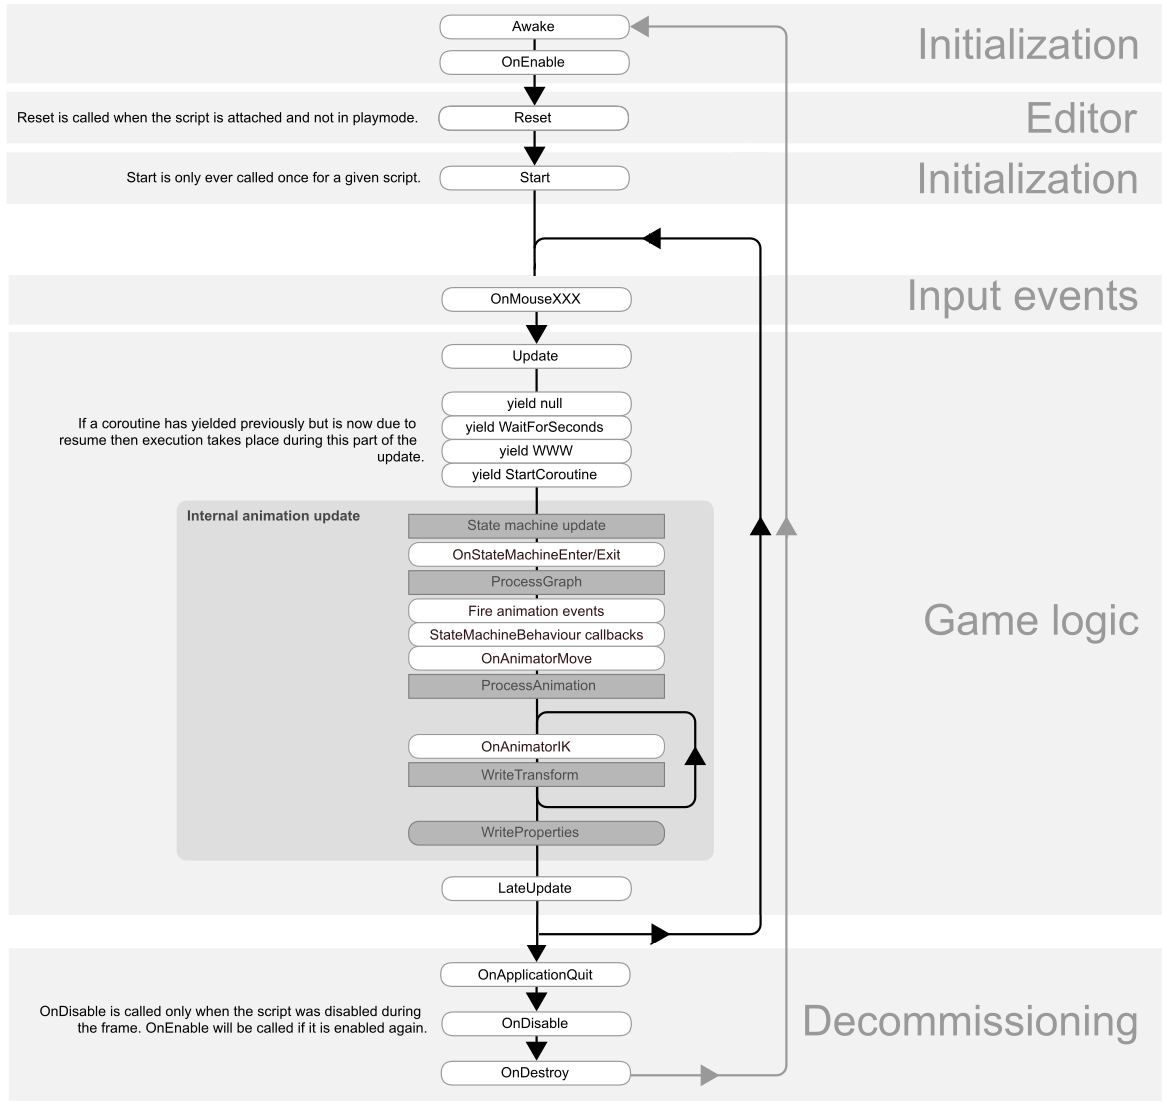
\includegraphics[scale = 0.4]{UnityEvents}
    \caption{Orden de ejecución para los eventos en Unity}
    \label{fig:UnityEvents} 
\end{figure} 

Las siguientes funciones, son algunas de las más importantes a la hora de desarrollar un escenario dentro de \textit{Unity}. Estas se llaman cuando una escena se ejecuta (una vez por cada objeto en la escena): 

\begin{itemize}
	\item \texttt{Awake}: esta función siempre se llama antes de cualquier función de inicio y también justo después de realizar una instancia de un \textit{prefab}.
 	\item \texttt{Start}: se llama al inicio antes de la actualización del primer marco solo si la instancia de secuencia de comandos está habilitada.
    \item \texttt{Update}: la actualización se llama una vez por fotograma. Es la principal función del motor para las actualizaciones de los \textit{frames}.
\end{itemize} 

Para construir todo el proyector de \textit{Unity} se utilizó el potente entorno de desarrollo \texttt{Visual Studio 2019}. 

\texttt{Visual Studio Tools} para \texttt{Unity} es una extensión gratuita de \texttt{Visual Studio} que convierte al editor en una poderosa herramienta para desarrollar juegos y aplicaciones multiplataforma con \texttt{Unity}.

Si bien el editor de \texttt{Unity} es excelente para crear el escenario 3D, pero no puedes escribir el código en él. Con \texttt{Visual Studio Tools} para \texttt{Unity}, se pueden usar las funciones familiares de edición, depuración y productividad de código para crear scripts en el proyecto de \texttt{Unity} usando C\#, pudiendo depurarlos usando las poderosas capacidades de depuración de \texttt{Visual Studio}.

Pero \texttt{Visual Studio Tools} para \texttt{Unity} es más que eso. También tiene una integración profunda con el editor de Unity para que dedique menos tiempo a realizar tareas simples, proporciona mejoras de productividad específicas de \texttt{Unity} y pone la documentación de al alcance de su mano.

\subsection{Adobe Fuse Character Creator}

Se trata de una aplicación desarrollada por Mixamo, la cual permite crear personajes 3D únicos mediante una intuitiva interfaz, separando el avatar en diferentes partes, como son la cabeza, el torso, las piernas y los brazos (véase Figura \ref{fig:AdobeFuse}). Posteriormente a la selección de las diferentes partes del cuerpo ya predefinidas por el sistema, se puede editar cada una de las partes del personaje, ya sean los rasgos de la cara, el tamaño de los brazos, la longitud de las piernas, etc. Al seleccionar la parte del cuerpo que se quiere modificar, simplemente sería necesario pinchar y realizar un \textit{scrool} o deslizamiento hacia la izquierda o derecha para aumentar su tamaño. Por otro lado, para seleccionar el punto exacto donde se ubicarán las diferentes partes del cuerpo como por ejemplo el ombligo, los ojos, las rodillas, etc, se realizará un \textit{scrool} o desplazamiento hacia arriba o abajo.

\begin{figure}[h!]
	\centering
	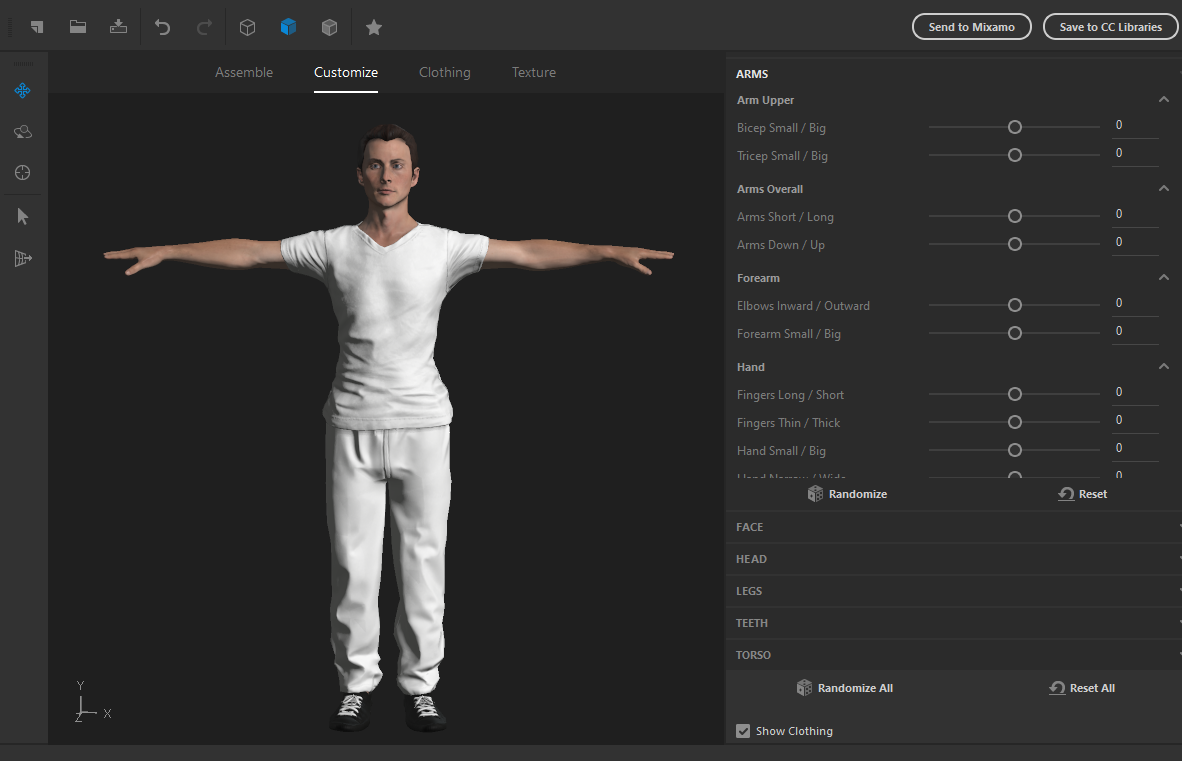
\includegraphics[scale = 0.4]{AdobeFuse}
	\caption{Configuración de un avatar con Adobe Fuse Character Creator}
	\label{fig:AdobeFuse}
\end{figure}

Al terminar de modelar el personaje, se pasará a la sección de vestuario. Donde existen prendas predefinidas, como camisas, pantalones, zapatos, etc. Al terminar de vestir al avatar, esta aplicación posee la peculiaridad de poder subir al servidor de Mixamo el modelado realizado \footnote{\url{https://www.adobe.com/es/products/fuse.html}}. Pudiendo completar la configuración de los huesos (\textit{rigger}), con la posibilidad de crear varios esqueletos para un mismo personaje y además incluir las animaciones deseadas.



\subsection{Mixamo}
\label{cap4:sec:mixamo}

Mixamo\footnote{\url{https://www.mixamo.com}} es una compañía tecnológica (adquirida en 2015 por Adobe System) encargada del desarrollo y venta de servicios para la animación de personajes 3D. Proporcionando un servicio \textit{online}, que permite buscar entre una amplia gama de movimientos, que van desde el combate, pasando por deportes, hasta poder tocar un instrumento (véase Figura \ref{fig:Mixamo}).

\begin{figure}[h]
    \centering 
    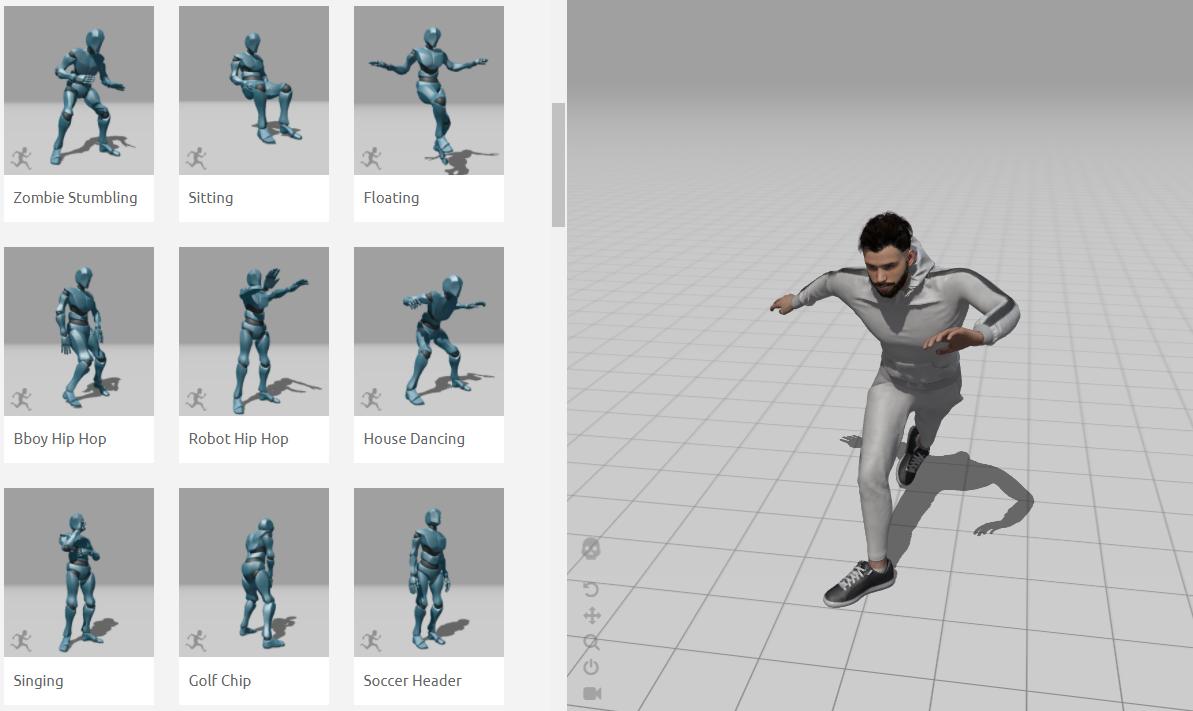
\includegraphics[scale = 0.4]{Mixamo}
    \caption{Servicio de animaciones de Mixamo}
    \label{fig:Mixamo} 
\end{figure} 

Los productos y características de Mixamo son compatibles con todos los paquetes de software 3D, pudiendo realizar una exportación, eligiendo entre varias aplicaciones 3D como: \texttt{Unity, Unreal Engine, Blender} y el conjunto de herramientas de Adobe Creative) entre otros.

Una de las características más sorprendentes de Mixamo, es el \textit{Auto-Rigger}. Ya que ahorras horas de trabajo modelando el personaje y con este sistema, el proceso sucede en cuestión de minutos. Todo lo que se necesita hacer es subir al servidor de Mixamo el personaje 3D (soporta .fbx, .bvh, .zip, obj), seleccionar el número de huesos que mejor se adapte al esqueleto del personaje y esperar que termine el proceso de \textit{rigger}.

Tras completar la fase de modelado, Mixamo ofrece la posibilidad de animar al personaje con movimientos, que permiten, no solo aplicar cualquier animación, sino también personalizarlas, ya que se pueden modificar en tiempo real con el personaje, obteniendo el resultado deseado. Por último, descargarlos en cualquier formato que se necesite (.fbx, .bvh, .dae) y fácilmente se podrá combinar de nuevo en las escenas 3D.

Estas animaciones utilizan una base matemática, lo que facilita su uso para los diferentes personajes que se deseen animar. Tradicionalmente era extremadamente lento, costoso y complicado, lograr modelar personajes 3D con resultados de alta calidad. En cambio, mediante esta técnica, Mixamo intenta reducir los tiempos de desarrollo, pudiendo obtener unas animaciones de calidad, sin la necesidad de contar con altos recursos. 

\section{Hardware empleado}
\label{cap4:sec:hardware empleado}

El hardware principal usado en este proyecto es el dispositivo de \textit{VR} \texttt{HTC Vive} capaz de conectar los diferentes sensores ópticos al ordenador con el sistema operativo Windows. Sin embargo, el desarrollo del proyecto se llevó a cabo en un ordenador de sobremesa, teniendo que utilizar unas características especiales de hardware capaces de mover gráficamente el sistema de \textit{VR}.

En cuanto al hardware utilizado para la otra aplicación desarrollada en este proyecto, se trata de un \textit{Smartphone} capaz de utilizar los sistemas más novedosos de \textit{ARCore}, como los sistemas de iluminación en tiempo real, los mapas de profundidad, entre otros.

\subsection{HTC Vive}

HTC Vive es un sistema de periféricos que se conectan al ordenador vía USB y HDMI o Displayport. La caja con el contenido de las HTC Vive es de grandes dimensiones, ya que trae un contenido extenso en su interior:

\begin{itemize}
    \item \texttt{ Gafas HTC Vive}: incluye un cable de alimentación, HDMI y USB de gran longitud, aproximadamente 5 metros.
    \item \texttt{ Link box}:caja de conexiones que conecta las gafas a un ordenador (enchufe de alimentación y su adaptador de luz, HDMI/Display y USB para PC además de las tres conexiones para las gafas)
	\item \texttt{ \textit{Sensores de posición / Base Station }}: incluyen dos unidades que requieren conexión a un enchufe y visión directa entre ellos. De manera opcional, conexión de cable directa entre sí.
    \item \texttt{Controles}: incluye dos unidades con carga vía microUSB, con cable y adaptador USB a enchufe cada uno.
    \item \texttt{ Auriculares minijack}: de cable corto con un pack de siliconas de distinto tamaño
    \item \texttt{\textit{Trackers}}: no se incluyen en el pack, pero para el desarrollo del proyecto se necesitan tres de ellos.
\end{itemize}

Para el correcto funcionamiento de HTC Vive, es necesario el uso de un ordenador potente para tener un una tasa de \textit{frames} de al menos 60fps.

\begin{itemize}
    \item \texttt{CPU}: Ryzen 7 3700x a 4.1GHz
    \item \texttt{RAM}: 16 GB DDR4
    \item \texttt{GPU}: Nvidia GeForce GTX 1660
    \item \texttt{Puertos USB}: un USB 3.0
    \item \texttt{SSD}: con al menos 128 GB dsponibles
    \item \texttt{Sistema Operativo}: Windows 10 Profesional
\end{itemize}

\subsection{Smartphone}

Los dispositivos Android a partir de la versión Android 7.0  son compatibles con algunas de las funcionalidades del sistema, a partir de la 10, es cuando se le puede sacar toda la potencia de este sistema.
\begin{itemize}
    \item \texttt{Marca y modelo}: Xiaomi Mi8
    \item \texttt{RAM}: 6 GB LPDDR4X
    \item \texttt{GPU}: Qualcomm Adreno 630 710MHz
    \item \texttt{Pantalla}: 6.21" Amoled
    \item \texttt{CPU}: Qualcomm Snapdragon 845 a 2.8GHz
    \item \texttt{Sistema Operativo}: Android 10
\end{itemize}